\chapter{iRRAM}
Die Software-Bibliothek \verb+iRRAM+ \cite{Mller2009EnhancingIE} basiert auf Intervallen als Zahlentyp, um diese mit einer beliebigen Genauigkeit darstellen zu können. Zunächst wird mit Double-Präzision (64-Bit Zahlen) gerechnet, welche verwendet werden, bis das Ergebnis für die angefragte Präzision nicht mehr genau ausgegeben werden kann, beziehungsweise bis zu einer bestimmten Anzahl an Bits. Ist dies der Fall, geschieht eine Iteration mit einer erhöhten Genauigkeit, also längeren Zahlen, welche dann mit Hilfe von \verb+MPFR+ dargestellt werden.
Für eine solche Iteration werden gerade so viele Zwischenergebnisse während der Berechnung gespeichert, dass eine Wiederholung der Schritte mit höherer Präzision möglich ist. Da nicht die gesamte Berechnung in jeder Iteration wiederholt wird, müssen während der Laufzeit Sichtbarkeit von Variablen und Zwischenergebnisse für den Nutzer genau kontrolliert und unter Umständen beschränkt werden, da sonst unerwartetes Verhalten und Exceptions entstehen können, indem die zugegriffenen Werte gegebenfall nicht in der aktuellen Iteration existieren.

\section{Verwendung der iRRAM-REALs}
Einige der für rationale Zahlen zur Verfügung stehenden Funktionen, wie der Vergleich zweier Zahlen, sind mit reellen Zahlen nicht ohne Weiteres Möglich. Dies gilt insbesondere für den Test auf Gleichheit und die Vorzeichenfunktion $sign$. Bei all diesen Funktionen handelt es sich im Reellen (und bei der \verb+iRRAM+) um mehrwertige Funktionen, da sich das jeweilige Ergebnis mit veränderter Präzsion in der Darstellung der Zahlen ändern kann. Dieses Problem wird in \verb+hotm+ durch den \verb+SignType+ adressiert. Zusätzlich zu den Werten 'positiv' (=\verb+POS+) und 'negativ' (=\verb+NEG+),  kann die Vorzeichenfunktion \verb+sign+ den Wert 'ambivalent' (=\verb+AMBI+) ausgeben, wenn nicht entscheidbar ist, wo genau die reelle Zahl um die Null liegt. Hierfür erhält die Vorzeichenfunktion einen Parameter, der den Bereich er Unsicherheit definiert. Ist der Ausgabewert 'ambivalent', so wird in den Funktionen, welche die Vorzeichenfunktion aufrufen, der schlechteste Fall im Hinblick auf die Genauigkeit des Ergebnisses angenommen. 


Eine weitere Besonderheit ergibt sich aus dem Aufbau der Zahlen, denn es entstehen zwei Intervall-`Ebenen`: Zum Einen, die Darstellung des Koeffizienten als Intervall aus Mitte und Radius. Zum Anderen die Darstellung von Mitte und Radius, als \verb+iRRAM-REAL+, also auch wiederum jeweils als Intervall mit Wert und Fehler, wie in Grafik \ref{fig:levels} zu sehen ist. Im Vergleich zu den \verb+mpq-RATIONALS+ erhöht sich hier zwar die Komplexität deutlich, allerdings lassen sich Ungenauigkeiten sehr genau steuern, indem zum Beispiel der Rechenfehler des Mittelpunkts eines Koeffizienten auf den Radius 'verlagert' wird. So vergrößert sich zwar der Radius des Koeffizienten, welcher dadurch ungenauer wird, jedoch verkleinert sich der Rechenfehler auf der Zahlenebene der \verb+REAL+s. Ein ählicher Effekt sollte sich durch Rundung auch mit den \verb+mpq-RATIONALS+ erreichen lassen. 


Das Verlagern der Ungenauigkeit ($e$ in der Grafik \ref{fig:levels}) auf den Wert des Radius' ($v$ in der Grafik), \textit{Micro-Housekeeping} genannt, verringert die Intervallbreite und erzeugt Punktintervalle auf der Zahlenebene, allerdings werden die Intervalle auf der Intervallebene breiter. Hier greift dann wiederum der Polish-Mechanismus, der auf Polynomebene Monome hinzufügt, um aus den zu groß gewordenen Intervallen wiederum Punktintervalle zu machen, \textit{Macro-Housekeeping} genannt. So wird der Rechenfehler von der untersten Ebene bis zur Polynomebene propagiert.
Diese Housekeeping-Funktionen werden durch Parameter gesteuert, die bestimmen, ab wann ein Intervall zu breit ist und die jeweilige Prozedur angewandt werden soll.

\begin{figure}[ht]
\label{fig:levels}
\begin{center}
 
 

\tikzset{every picture/.style={line width=0.75pt}} %set default line width to 0.75pt        

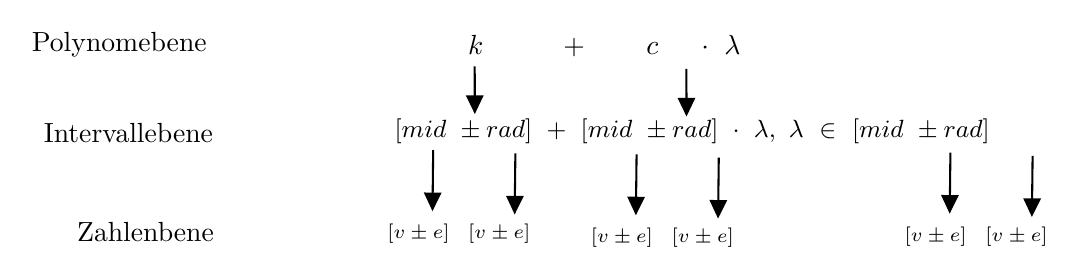
\begin{tikzpicture}[x=0.75pt,y=0.75pt,yscale=-1,xscale=1]
%uncomment if require: \path (0,300); %set diagram left start at 0, and has height of 300

%Straight Lines [id:da29898159624783616] 
\draw    (281.07,90.5) -- (280.77,116.88) ;
\draw [shift={(280.73,119.88)}, rotate = 270.65] [fill={rgb, 255:red, 0; green, 0; blue, 0 }  ][line width=0.08]  [draw opacity=0] (8.93,-4.29) -- (0,0) -- (8.93,4.29) -- cycle    ;
%Straight Lines [id:da1335093356184387] 
\draw    (320.67,92.1) -- (320.37,118.48) ;
\draw [shift={(320.33,121.48)}, rotate = 270.65] [fill={rgb, 255:red, 0; green, 0; blue, 0 }  ][line width=0.08]  [draw opacity=0] (8.93,-4.29) -- (0,0) -- (8.93,4.29) -- cycle    ;
%Straight Lines [id:da1340726243132735] 
\draw    (379.07,92.5) -- (378.77,118.88) ;
\draw [shift={(378.73,121.88)}, rotate = 270.65] [fill={rgb, 255:red, 0; green, 0; blue, 0 }  ][line width=0.08]  [draw opacity=0] (8.93,-4.29) -- (0,0) -- (8.93,4.29) -- cycle    ;
%Straight Lines [id:da9182990047680641] 
\draw    (418.67,94.1) -- (418.37,120.48) ;
\draw [shift={(418.33,123.48)}, rotate = 270.65] [fill={rgb, 255:red, 0; green, 0; blue, 0 }  ][line width=0.08]  [draw opacity=0] (8.93,-4.29) -- (0,0) -- (8.93,4.29) -- cycle    ;
%Straight Lines [id:da04610901450657834] 
\draw    (530.27,91.7) -- (529.97,118.08) ;
\draw [shift={(529.93,121.08)}, rotate = 270.65] [fill={rgb, 255:red, 0; green, 0; blue, 0 }  ][line width=0.08]  [draw opacity=0] (8.93,-4.29) -- (0,0) -- (8.93,4.29) -- cycle    ;
%Straight Lines [id:da7044032296577734] 
\draw    (569.87,93.3) -- (569.57,119.68) ;
\draw [shift={(569.53,122.68)}, rotate = 270.65] [fill={rgb, 255:red, 0; green, 0; blue, 0 }  ][line width=0.08]  [draw opacity=0] (8.93,-4.29) -- (0,0) -- (8.93,4.29) -- cycle    ;
%Straight Lines [id:da7628093943540135] 
\draw    (301.07,50.1) -- (301.12,70.08) ;
\draw [shift={(301.13,73.08)}, rotate = 269.84000000000003] [fill={rgb, 255:red, 0; green, 0; blue, 0 }  ][line width=0.08]  [draw opacity=0] (8.93,-4.29) -- (0,0) -- (8.93,4.29) -- cycle    ;
%Straight Lines [id:da9018979196177348] 
\draw    (403.07,51.3) -- (403.12,71.28) ;
\draw [shift={(403.13,74.28)}, rotate = 269.84000000000003] [fill={rgb, 255:red, 0; green, 0; blue, 0 }  ][line width=0.08]  [draw opacity=0] (8.93,-4.29) -- (0,0) -- (8.93,4.29) -- cycle    ;

% Text Node
\draw (86.2,32) node [anchor=north west][inner sep=0.75pt]   [align=left] {Polynomebene};
% Text Node
\draw (92,76) node [anchor=north west][inner sep=0.75pt]   [align=left] {Intervallebene};
% Text Node
\draw (108,124) node [anchor=north west][inner sep=0.75pt]   [align=left] {Zahlenbene};
% Text Node
\draw (296.4,33.8) node [anchor=north west][inner sep=0.75pt]    {$k\ \ \ \ \ \ \ \ +\ \ \ \ \ \  c\ \ \ \ \cdot \ \lambda $};
% Text Node
\draw (261,74) node [anchor=north west][inner sep=0.75pt]  [font=\small]  {$\left[\text{mid} \ \pm \text{rad}\right] \ +\ \left[\text{mid} \ \pm \text{rad}\right] \ \cdot \ \lambda ,\ \lambda \ \in \ \left[\text{mid} \ \pm \text{rad}\right]$};
% Text Node
\draw (257.5,124.6) node [anchor=north west][inner sep=0.75pt]  [font=\scriptsize]  {$\left[\text{v} \pm \text{e}\right] \ \ \left[\text{v} \pm \text{e}\right]$};
% Text Node
\draw (355.5,126.6) node [anchor=north west][inner sep=0.75pt]  [font=\scriptsize]  {$\left[\text{v} \pm \text{e}\right] \ \ \left[\text{v} \pm \text{e}\right]$};
% Text Node
\draw (506.7,125.8) node [anchor=north west][inner sep=0.75pt]  [font=\scriptsize]  {$\left[\text{v} \pm \text{e}\right] \ \ \left[\text{v} \pm \text{e}\right]$};


\end{tikzpicture}

 \caption{Ebenen der Polynomdarstellung mit REALs (informell)}
 \end{center}
\end{figure}


\section{Genauigkeitsmodell}
\label{sec:precision}
Die \verb+iRRAM+ bietet die Möglichkeit, zwischen \textit{absoluter} und \textit{relativer} Genauigkeit zu unterscheiden. Absolute Genauigkeit bedeutet, dass beim Verrechnen zweier \verb+REAL+s ein global verwendeter Wert für die Genauigkeit zugrunde liegt und die Zahlen dementsprechen skaliert werden. Bei relativer Genauigkeit hängt die verwendete Genauigkeit von der tatsächlichen Größe der jeweiligen Zahlen ab. Diese kann zum Beispiel durch punktuelle Anwendung von Micro-Housekeeping stark variieren, weshalb die Verwendung von relativer Genauigkeit in der Praxis besser funktioniert.


Für der Vergleich wurde $x_{1000}$ mit $x_n = c \cdot x_{n-1} \cdot (1 - x_{n-1})$ mit der folgenden Konfiguration berechnet:
\begin{enumerate}
 \item Nur quadratisches Sweeping zur 0,
 \item Micro-Housekeeping (Cleaning) ab einem Fehler $\chi$ auf Zahlenebene $>10^{-100}$,
 \item Macro-Housekeeping (Polish) ab einer Intervallbreite $\psi$ $>10^{-50}$,
 \item $x_0 = 0,5$ und
 \item Ausgabe des Ergebnisses auf 20 Stellen genau.
\end{enumerate}
Zu Beginn einer jeden Iteration wird zunächst gesweept (1.), dann der Fehler und die Intervalle bereinigt (2.) und zuletzt das Polynom poliert (3.), bevor erneut multipliziert wird. Für $c = 3.25$ konvergiert die Funktion gegen zwei Werte und lässt sich sehr genau bestimmen.

\begin{center}
\begin{tabular}{|r|c|c|}
\hline
\multicolumn{3}{|c|}{$x_{1000}$ mit $c=3.25$}\\
\hline
 mit Housekeeping&relative Genauigkeit & absolute Genauigkeit \\
 \hline
 \hline
 Anzahl Polishs & 142 & 6961 \\
 Präzision (Bits) & \verb+double+ & 136 \\
 CPU-Zeit & 0.8s & 4.43s\\
 \hline
\end{tabular}
\end{center}

Wie in der Tabelle zu sehen ist, benötigt die Berechnung mit relativer Genauigkeit erheblich weniger Zeit und Bits um ein Ergebnis mit der geforderten Auflösung zu erhalten. Wird auf die Housekeeping-Methoden verzichtet, zeigt sich dieser massive Unterschied jedoch nicht:

\begin{center}
\begin{tabular}{|r|c|c|}
\hline
\multicolumn{3}{|c|}{$x_{1000}$ mit $c=3.25$}\\
\hline
 ohne Housekeeping &relative Genauigkeit & absolute Genauigkeit \\
 \hline
 \hline
 Anzahl Polishs & -& -\\
 Präzision (Bits) & 7440 & 7440 \\
 CPU-Zeit & 0.120s & 0.118s\\
 \hline
\end{tabular}
\end{center}

Die Ergenisse werden ohne Housekeeping erheblich schneller berechnet, allerdings auf Kosten der benötigten Bits für die Zahlendarstellung. Da hier kein Polieren geschieht, wird auch kein Taylormodell als solches initialisiert, das heißt, es werden keine Fehlersymbole eingesetzt und rein auf der Ebene der reellen Zahlen der \verb+iRRAM+ gerechnet.

Für $c=3.75$, einem Wert, bei dem die Funktion chaotisches Verhalten aufweist und zwischen vielen Werten hin- und herspringt, ist erkennbar, dass ein Rechnen mit diesen Housekeeping-Parametern und absoluter Genauigkeit nicht praktikabel ist, da die Berechnung bereits nach 64 Iterationen eine Laufzeit von über 15 Sekunden hat, welche scheinbar exponentiell steigt. Für relative Genauigkeit is die Berechnung zwar zeitaufwändiger, liefert jedoch ein (korrektes) Ergebnis.

\begin{center}
\begin{tabular}{|r|c|c|}
\hline
\multicolumn{3}{|c|}{$x_{1000}$ mit $c=3.75$}\\
\hline
 mit Housekeeping &relative Genauigkeit & absolute Genauigkeit \\
 \hline
 \hline
 Anzahl Polishs & 5511 & ?\\
 Präzision (Bits) & 7440 & ?\\
 CPU-Zeit & 4.02s & >60s\\
 \hline
\end{tabular}
\end{center}

Wie oben zeigt sich zwischen relativer und absoluter Genauigkeit bei der Verwendung ohne Housekeeping-Methoden kein nennenswerter Unterschied. Zudem scheint bei der hier verwendeten Konfiguration lediglich ein Berechnungsoverhead zu entstehen, welcher keine Auswirkungen auf die Qualität des Ergebnisses hat.


\begin{center}
\begin{tabular}{|r|c|c|}
\hline
\multicolumn{3}{|c|}{$x_{1000}$ mit $c=3.75$}\\
\hline
 ohne Housekeeping &relative Genauigkeit & absolute Genauigkeit \\
 \hline
 \hline
 Anzahl Polishs & - & -\\
 Präzision (Bits) & 7440 & 7440\\
 CPU-Zeit & 0.12s & 0.12s\\
 \hline
\end{tabular}
\end{center}


Insgesamt lässt sich beobachten, dass die Berechnung der Interationen mit relativer Genauigkeit in den untersuchten Fällen bessere Ergebnisse liefert, weshalb diese im Folgenden zugrunde liegt.

\section{Housekeeping}
Die Werte der Parameter für die Housekeeping-Methoden hängen unmittelbar voneinander ab: Je größer der Wert des Cleaning $\chi$, also as Umlagern des Rechenfehlers eines Koeffizienten auf den Mittelpunkt des Radius', desto schneller wird der Grenzwert des Polishs $\psi$, also des Einführens eines neuen Fehlersymbols erreicht.

Für $c=3.25$ kann $x_{1000}$ mit $\psi = 10^{-50}$ in \verb+double+ -Präzision berechnet werden, solange $\psi \geq \chi$ gilt. Je mehr sich $\psi$ und $\chi$ annähern, desto öfter überschreitet der Radius eines Koeffizienten den Grenzwert $\psi$ und wird poliert, wie in Grafik \ref{fig:polish} zu sehen ist.

\begin{figure}[ht]
    \centering
    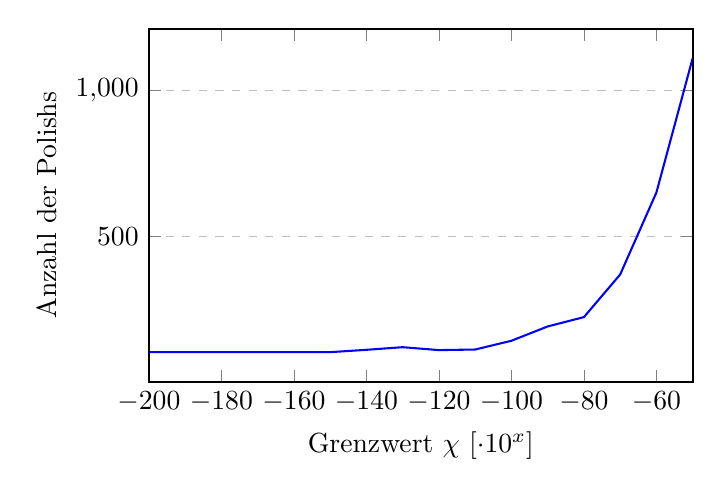
\begin{tikzpicture}
    \begin{axis}[
    width=0.7\textwidth,
    height=0.5\textwidth,
        xlabel={Grenzwert $\chi$ [$\cdot 10^{x}$]},
        ylabel={Anzahl der Polishs},
        legend pos=north west,
        xmin=-200,xmax=-50,
        ymajorgrids=true,
        grid style=dashed
    ]
    \addplot[
        color=blue,
        ]
        coordinates {
(-200,103)
(-190,103)
(-180,103)
(-170,103)
(-160,103)
(-150,103)
(-140,111)
(-130,120)
(-120,110)
(-110,112)
(-100,142)
(-90,191)
(-80,223)
(-70,369)
(-60,650)
(-50,1110)
        };

        
    \end{axis}
    \end{tikzpicture}
    \caption[Grenzwertvergleich]{Anzahl der Polishs für $x_{1000}$ bei \\ $\psi = 10^{-50}$ und wachsendem $\chi$}
    \label{fig:polish}
\end{figure}

Wird stattdessen $\chi>\psi$ definiert, so erhöht sich weiterhin die Anzahl der Polishs, als auch die benötigten Bits für die Ausgabe des Ergebnisses:


\begin{center}
\begin{tabular}{|c|c|c|c|}
\hline
\multicolumn{4}{|c|}{$x_{1000}$ mit $c=3.75$}\\
\hline
 $\psi$ & $\chi$ & Bits & Polishs\\
 \hline
    & $10^{-50}$ & \verb+double+ & 1110 \\
    & $10^{-40}$ & 2876 & 2907\\
$10^{-50}$& $10^{-30}$ & 2876 & 3890\\
    & $10^{-25}$ & 2876 & 5542\\ 
    & $10^{-24}$ & 2876 & 5998\\ 
    & $10^{-20}$ & 375 & 1594\\
    & $10^{-15}$ & 2876 & 72\\
    & $10^{-10}$ & 2876 &103\\
    & $10^{-5}$ & 7440 & 0\\
 \hline
\end{tabular}
\end{center}



Ab einer bestimmten 

\begin{landscape}
\begin{table}

 
 \small

\renewcommand{\arraystretch}{1.2}
\begin{tabular}{|c|c|c|c|c|c|c|c|c|c|c|c|}
\hline
  \begin{tabular}[t]{@{}lr@{}}
      $\cdot 10^{-x}$     & $\psi$  \\
     $\chi$&
  \end{tabular}& 0 & 10 & 20 & 30 & 40 & 50 & 60 & 70 & 80 & 90& 100 \\
\hline 
0&
\shortstack{ \\7440\\ 0\\ 1.6326 s}& 
\shortstack{ \\7440\\ 0\\ 1.83337 s}& 
\shortstack{ \\7440\\ 0\\ 1.94407 s}& 
\shortstack{ \\7440\\ 0\\ 2.04077 s}& 
\shortstack{ \\7440\\ 0\\ 2.11908 s}& 
\shortstack{ \\7440\\ 0\\ 2.21374 s}& 
\shortstack{ \\7440\\ 0\\ 2.29907 s}& 
\shortstack{ \\7440\\ 0\\ 2.38224 s}& 
\shortstack{ \\7440\\ 0\\ 2.467 s}& 
\shortstack{ \\7440\\ 0\\ 2.55054 s}& 
\shortstack{ \\7440\\ 0\\ 2.63597 s} \\
\hline
10&
\shortstack{ \\7440\\ 0\\ 2.78598 s}& 
\shortstack{ \\9372\\ 0\\ 5.52392 s}& 
\shortstack{ \\2876\\ 172\\ 5.02589 s}& 
\shortstack{ \\2876\\ 124\\ 5.00488 s}& 
\shortstack{ \\2876\\ 113\\ 5.07724 s}& 
\shortstack{ \\2876\\ 103\\ 5.54921 s}& 
\shortstack{ \\2876\\ 101\\ 5.35356 s}& 
\shortstack{ \\2876\\ 107\\ 5.4392 s}& 
\shortstack{ \\2876\\ 124\\ 5.68067 s}& 
\shortstack{ \\2876\\ 130\\ 5.85416 s}& 
\shortstack{ \\2876\\ 142\\ 6.06347 s}\\ 
\hline
20&
\shortstack{ \\7440\\ 0\\ 3.94074 s}& 
\shortstack{ \\242\\ 1277\\ 8.10701 s}& 
\shortstack{ \\50\\ 2780\\ 4.72946 s}& 
\shortstack{ \\748\\ 565\\ 9.75293 s}& 
\shortstack{ \\748\\ 555\\ 8.68541 s}& 
\shortstack{ \\375\\ 1594\\ 8.93876 s}& 
\shortstack{ \\375\\ 1880\\ 25.4399 s}& 
\shortstack{ \\748\\ 913\\ 22.1312 s}& 
\shortstack{ \\1008\\ 672\\ 26.4569 s}& 
\shortstack{ \\375\\ 2790\\ 36.9133 s}& 
\shortstack{ \\1008\\ 793\\ 35.4304 s}\\
\hline
30&
\shortstack{ \\7440\\ 0\\ 13.1344 s}& 
\shortstack{ \\242\\ 1231\\ 24.1473 s}& 
\shortstack{ \\2876\\ 178\\ 49.0635 s}& 
\shortstack{ \\2876\\ 103\\ 80.8316 s}& 
\shortstack{ \\2876\\ 78\\ 184.06 s}& 
\shortstack{ \\2876\\ 74\\ 250.773 s}& 
\shortstack{ \\2876\\ 55\\ 365.989 s}& 
\shortstack{ \\2876\\ 51\\ 511.508 s}& 
\shortstack{ \\2876\\ 49\\ 684.393 s}& 
\shortstack{ \\2876\\ 51\\ 848.406 s}& 
\shortstack{ \\2876\\ 55\\ 997.68 s}\\
\hline
40&
\shortstack{ \\7440\\ 0\\ 53.3362 s}& 
\shortstack{ \\50\\ 1256\\ 29.1948 s}& 
\shortstack{ \\2876\\ 176\\ 99.8966 s}& 
\shortstack{ \\2876\\ 103\\ 125.306 s}& 
\shortstack{ \\748\\ 830\\ 143.597 s}& 
\shortstack{ \\2876\\ 59\\ 478.68 s}& 
\shortstack{ \\2876\\ 51\\ 529.705 s}& 
\shortstack{ \\2876\\ 48\\ 629.886 s}& 
\shortstack{ \\2876\\ 45\\ 861.242 s}& 
\shortstack{ \\2876\\ 47\\ 937.462 s}& 
\shortstack{ \\1008\\ 3249\\ 970.695 s}\\
\hline
50&
\shortstack{ \\7440\\ 0\\ 75.4545 s}& 
\shortstack{ \\541\\ 1092\\ 197.334 s}& 
\shortstack{ \\2876\\ 157\\ 102.602 s}& 
\shortstack{ \\2876\\ 100\\ 105.98 s}& 
\shortstack{ \\136\\ 626\\ 42.8746 s}& 
\shortstack{ \\50\\ 1110\\ 36.735 s}& 
\shortstack{ \\50\\ 2058\\ 67.4805 s}& 
\shortstack{ \\50\\ 3061\\ 99.8092 s}& 
\shortstack{ \\50\\ 3104\\ 101.562 s}& 
\shortstack{ \\50\\ 3252\\ 106.672 s}& 
\shortstack{ \\50\\ 4307\\ 141.643 s}\\
\hline
60&
\shortstack{ \\7440\\ 0\\ 77.9164 s}& 
\shortstack{ \\50\\ 1330\\ 44.7121 s}& 
\shortstack{ \\2876\\ 197\\ 109.461 s}& 
\shortstack{ \\2876\\ 102\\ 77.7069 s}& 
\shortstack{ \\50\\ 360\\ 12.852 s}& 
\shortstack{ \\50\\ 650\\ 22.519 s}& 
\shortstack{ \\50\\ 793\\ 27.3169 s}& 
\shortstack{ \\50\\ 1478\\ 49.8977 s}& 
\shortstack{ \\50\\ 2831\\ 94.8471 s}& 
\shortstack{ \\50\\ 3006\\ 101.299 s}& 
\shortstack{ \\50\\ 3046\\ 102.522 s}\\
\hline
70&
\shortstack{ \\7440\\ 0\\ 78.5848 s}& 
\shortstack{ \\50\\ 1209\\ 41.5528 s}& 
\shortstack{ \\50\\ 305\\ 11.2421 s}& 
\shortstack{ \\50\\ 182\\ 7.14775 s}& 
\shortstack{ \\50\\ 244\\ 9.10952 s}& 
\shortstack{ \\50\\ 369\\ 13.3082 s}& 
\shortstack{ \\50\\ 585\\ 20.5524 s}& 
\shortstack{ \\50\\ 730\\ 25.4535 s}& 
\shortstack{ \\50\\ 1498\\ 51.1763 s}& 
\shortstack{ \\50\\ 2198\\ 74.7332 s}& 
\shortstack{ \\50\\ 3052\\ 103.7 s}\\
\hline
80&
\shortstack{ \\7440\\ 0\\ 80.0082 s}& 
\shortstack{ \\50\\ 1265\\ 44.0294 s}& 
\shortstack{ \\50\\ 283\\ 10.6252 s}& 
\shortstack{ \\50\\ 209\\ 8.17959 s}& 
\shortstack{ \\50\\ 193\\ 7.62534 s}& 
\shortstack{ \\50\\ 223\\ 8.50545 s}& 
\shortstack{ \\50\\ 346\\ 12.6874 s}& 
\shortstack{ \\50\\ 618\\ 21.9991 s}& 
\shortstack{ \\50\\ 619\\ 21.985 s}& 
\shortstack{ \\50\\ 2099\\ 72.5467 s}& 
\shortstack{ \\50\\ 2540\\ 87.2578 s}\\ 
\hline
90&
\shortstack{ \\7440\\ 0\\ 81.4708 s}& 
\shortstack{ \\50\\ 1279\\ 44.8837 s}& 
\shortstack{ \\50\\ 285\\ 10.7928 s}& 
\shortstack{ \\50\\ 179\\ 7.13232 s}& 
\shortstack{ \\50\\ 133\\ 5.57989 s}& 
\shortstack{ \\50\\ 191\\ 7.4692 s}& 
\shortstack{ \\50\\ 229\\ 8.78794 s}& 
\shortstack{ \\50\\ 365\\ 13.5734 s}& 
\shortstack{ \\50\\ 651\\ 23.2493 s}& 
\shortstack{ \\50\\ 851\\ 30.1336 s}& 
\shortstack{ \\50\\ 1760\\ 61.3092 s}\\
\hline
100&
\shortstack{ \\7440\\ 0\\ 83.1739 s}& 
\shortstack{ \\50\\ 1181\\ 42.1948 s}& 
\shortstack{ \\50\\ 332\\ 12.458 s}& 
\shortstack{ \\50\\ 184\\ 7.5799 s}& 
\shortstack{ \\50\\ 134\\ 5.65369 s}& 
\shortstack{ \\50\\ 142\\ 5.86399 s}& 
\shortstack{ \\50\\ 199\\ 7.81504 s}& 
\shortstack{ \\50\\ 236\\ 9.11688 s}& 
\shortstack{ \\50\\ 391\\ 14.4456 s}& 
\shortstack{ \\50\\ 571\\ 20.7529 s}& 
\shortstack{ \\50\\ 709\\ 25.5848 s}\\
\hline
\end{tabular}

\caption[Kombinationsmöglichkeiten der Grenzwerte für Housekeeping-Methoden]{Kombinationsmöglichkeiten der Grenzwerte für Housekeeping-Methoden. Die Zelle besteht aus den benötigten Bits für die Ausgabe, der Anzahl der Polishs und der CPU-Zeit für die Berechnung von $x_{1000}$ für $c=3.25$, wie in Kapitel \ref{sec:precision} beschrieben}
\label{tab:thresholds}
\end{table}
\end{landscape}
% 
% \begin{table}[ht]
%     \centering
%     \def\arraystretch{1.3}
%     \begin{tabular}{r|c|c|c}
%     Iterationen &Metrik & absolut & relativ \\
%     \hline
%     $n=60$ & CPU-Zeit & $0.08s$ &  $3.21s$       \\
%            & Genauigkeit & \verb+double+ &   $2^{-748}$      \\
%            & Anzahl Polishs & 45 &    374     \\ 
%     \hline
%     $n=65$ & CPU-Zeit & $0.14s$ &  $18.06s$       \\
%            & Genauigkeit & \verb+double+ &  $2^{-748}$       \\
%            & Anzahl Polishs & 71 &   409      \\
%     \hline
%     $n=66$ & CPU-Zeit & $0.18s$ & $69s$\\
%            & Genauigkeit & \verb+double+ &   $2^{-748}$      \\
%            & Anzahl Polishs & 77 &    416     \\
%     \hline
%     $n=67$ & CPU-Zeit & $0.23s$ & $180s$ \\
%            & Genauigkeit & \verb+double+ &   $2^{-748}$      \\
%            & Anzahl Polishs & 84 &     423    \\
%     \hline
%     $n=100$ & CPU-Zeit & $0.38s$ & $>180s$ \\
%            & Genauigkeit & $2^{-748}$ &??\\
%            & Anzahl Polishs & 314 &??\\
%     \hline
%     $n=500$ & CPU-Zeit & $2.83s$ &$>180s$\\
%            & Genauigkeit & $2^{-2876}$ &??\\
%            & Anzahl Polishs & 3939 &??\\
%     \end{tabular}
%     \caption[Vergleich von Genauigkeitsmodellen]{Vergleich vom Rechnen mit absoluter und relativer Genauigkeit}
%     \label{tab:precision}
% \end{table}
